% =============================================================================
% Chapter 9: The Training Loop
% =============================================================================
\chapter{The Training Loop}
\label{ch:training-loop}

\begin{objectives}
    \item Understand the complete training loop structure
    \item Learn about AdamW optimizer and weight decay
    \item Master gradient accumulation for larger effective batches
    \item Understand mixed precision training
    \item Implement gradient clipping for stability
    \item Learn about learning rate schedules
\end{objectives}

% -----------------------------------------------------------------------------
\section{Training Loop Overview}
% -----------------------------------------------------------------------------

Training a neural network is an iterative optimization process:

\begin{enumerate}
    \item \textbf{Forward pass}: Compute predictions and loss
    \item \textbf{Backward pass}: Compute gradients via backpropagation
    \item \textbf{Optimizer step}: Update weights to reduce loss
    \item \textbf{Repeat}: Until convergence or max steps
\end{enumerate}

\begin{figure}[H]
\centering
\begin{tikzpicture}[
    box/.style={rectangle, draw, rounded corners, minimum width=3cm, minimum height=0.8cm, fill=blue!10},
    arrow/.style={-{Stealth[length=2mm]}, thick},
]
    % Boxes
    \node[box] (data) at (0, 0) {Get Batch};
    \node[box] (forward) at (4, 0) {Forward Pass};
    \node[box] (loss) at (8, 0) {Compute Loss};
    \node[box] (backward) at (8, -2) {Backward Pass};
    \node[box] (update) at (4, -2) {Update Weights};
    \node[box] (log) at (0, -2) {Log Metrics};

    % Arrows
    \draw[arrow] (data) -- (forward);
    \draw[arrow] (forward) -- (loss);
    \draw[arrow] (loss) -- (backward);
    \draw[arrow] (backward) -- (update);
    \draw[arrow] (update) -- (log);
    \draw[arrow] (log) -- (data);

    % Labels
    \node[font=\footnotesize, gray, above=0.1cm of forward] {model(batch)};
    \node[font=\footnotesize, gray, below=0.1cm of backward] {loss.backward()};
    \node[font=\footnotesize, gray, below=0.1cm of update] {optimizer.step()};
\end{tikzpicture}
\caption{The training loop cycle}
\label{fig:training-loop}
\end{figure}

% -----------------------------------------------------------------------------
\section{The AdamW Optimizer}
% -----------------------------------------------------------------------------

\TryLM uses \textbf{AdamW}, the standard optimizer for transformer training.

\subsection{Adam: Adaptive Moments}

Adam maintains two moving averages for each parameter:
\begin{itemize}
    \item \textbf{First moment} ($m$): Exponential moving average of gradients
    \item \textbf{Second moment} ($v$): Exponential moving average of squared gradients
\end{itemize}

\begin{align}
m_t &= \beta_1 m_{t-1} + (1 - \beta_1) g_t \\
v_t &= \beta_2 v_{t-1} + (1 - \beta_2) g_t^2 \\
\theta_t &= \theta_{t-1} - \alpha \cdot \frac{\hat{m}_t}{\sqrt{\hat{v}_t} + \epsilon}
\end{align}

\subsection{AdamW: Decoupled Weight Decay}

AdamW separates weight decay from the gradient-based update:

\begin{equation}
\theta_t = \theta_{t-1} - \alpha \cdot \left( \frac{\hat{m}_t}{\sqrt{\hat{v}_t} + \epsilon} + \lambda \theta_{t-1} \right)
\end{equation}

\begin{keypoint}
\textbf{Weight decay} ($\lambda$) shrinks weights toward zero, acting as regularization. AdamW applies it separately from the adaptive learning rate, which empirically works better than L2 regularization.
\end{keypoint}

\subsection{Differential Weight Decay}

Not all parameters should have weight decay. We apply it only to weight matrices, not biases or normalization parameters:

\begin{lstlisting}[style=python, caption={Optimizer configuration from trainer.py}]
def _configure_optimizer(self) -> torch.optim.Optimizer:
    # Separate parameters into decay and no-decay groups
    decay_params = []
    no_decay_params = []

    for name, param in self.model.named_parameters():
        if not param.requires_grad:
            continue

        # Don't decay biases, embeddings, or normalization weights
        if param.ndim < 2 or "embedding" in name:
            no_decay_params.append(param)
        else:
            decay_params.append(param)

    optimizer = torch.optim.AdamW([
        {"params": decay_params, "weight_decay": self.config.weight_decay},
        {"params": no_decay_params, "weight_decay": 0.0},
    ],
        lr=self.config.learning_rate,  # 3e-4
        betas=(0.9, 0.95),
        eps=1e-8,
    )
    return optimizer
\end{lstlisting}

\subsection{Why Different Betas?}

\TryLM uses $\beta_1 = 0.9$ and $\beta_2 = 0.95$ (instead of the default 0.999):
\begin{itemize}
    \item Lower $\beta_2$ makes the optimizer more responsive to recent gradients
    \item This helps with the non-stationary optimization landscape of transformers
\end{itemize}

% -----------------------------------------------------------------------------
\section{Gradient Accumulation}
% -----------------------------------------------------------------------------

GPU memory limits batch size. \textbf{Gradient accumulation} simulates larger batches.

\subsection{The Problem}

Larger batches generally lead to more stable training:
\begin{itemize}
    \item Gradient estimates are less noisy
    \item Enables larger learning rates
\end{itemize}

But GPU memory limits how many sequences we can process at once.

\subsection{The Solution}

Instead of one large batch, process multiple small batches and accumulate gradients:

\begin{lstlisting}[style=python]
# Effective batch = batch_size * gradient_accumulation_steps
# 256 = 64 * 4

for step in range(max_steps):
    optimizer.zero_grad()

    # Accumulate gradients over multiple micro-batches
    for micro_step in range(gradient_accumulation_steps):
        batch = next(data_iter)
        loss = model(batch)["loss"]

        # Scale loss by accumulation steps
        (loss / gradient_accumulation_steps).backward()

    # Update weights once per effective batch
    optimizer.step()
\end{lstlisting}

\begin{figure}[H]
\centering
\begin{tikzpicture}[
    box/.style={rectangle, draw, minimum width=1.5cm, minimum height=0.8cm, fill=blue!10},
    acc/.style={rectangle, draw, minimum width=1.5cm, minimum height=0.8cm, fill=orange!20},
    arrow/.style={-{Stealth[length=2mm]}, thick},
]
    % Micro batches
    \node[box] (b1) at (0, 0) {Batch 1};
    \node[box] (b2) at (2, 0) {Batch 2};
    \node[box] (b3) at (4, 0) {Batch 3};
    \node[box] (b4) at (6, 0) {Batch 4};

    % Gradient accumulation
    \node[acc, minimum width=6.5cm] (acc) at (3, -1.5) {Accumulated Gradients};

    % Optimizer step
    \node[box, fill=green!20, minimum width=3cm] (step) at (3, -3) {Optimizer Step};

    % Arrows
    \foreach \b in {b1, b2, b3, b4} {
        \draw[arrow] (\b) -- (acc);
    }
    \draw[arrow] (acc) -- (step);

    % Labels
    \node[font=\footnotesize, gray] at (3, -0.7) {backward() on each};
    \node[font=\footnotesize, gray] at (3, -2.3) {step() once};
\end{tikzpicture}
\caption{Gradient accumulation: 4 batches contribute to one optimizer step}
\label{fig:gradient-accumulation}
\end{figure}

\begin{keypoint}
With batch\_size=64 and gradient\_accumulation\_steps=4, the \textbf{effective batch size} is $64 \times 4 = 256$ sequences.
\end{keypoint}

% -----------------------------------------------------------------------------
\section{Mixed Precision Training}
% -----------------------------------------------------------------------------

\textbf{Mixed precision} uses lower-precision (float16/bfloat16) for most computations while maintaining float32 for critical operations.

\subsection{Benefits}

\begin{enumerate}
    \item \textbf{Faster}: GPUs compute float16 much faster
    \item \textbf{Less memory}: Half the bytes per number
    \item \textbf{Larger batches}: More sequences fit in memory
\end{enumerate}

\subsection{Challenges}

Float16 has limited range ($\sim 10^{-5}$ to $\sim 65504$):
\begin{itemize}
    \item Gradients can underflow (become zero)
    \item Weights updates may be too small to represent
\end{itemize}

\subsection{Loss Scaling}

\textbf{GradScaler} automatically scales the loss to prevent underflow:

\begin{lstlisting}[style=python, caption={Mixed precision training from trainer.py}]
from torch.cuda.amp import autocast, GradScaler

# Create scaler
scaler = GradScaler() if mixed_precision else None

for batch in dataloader:
    optimizer.zero_grad()

    # Forward pass in mixed precision
    with autocast(enabled=mixed_precision):
        outputs = model(**batch)
        loss = outputs["loss"] / gradient_accumulation_steps

    # Backward with scaled loss
    if scaler is not None:
        scaler.scale(loss).backward()
    else:
        loss.backward()

    # Optimizer step with unscaling
    if scaler is not None:
        scaler.unscale_(optimizer)
        # Gradient clipping here
        scaler.step(optimizer)
        scaler.update()
    else:
        optimizer.step()
\end{lstlisting}

\begin{keypoint}
\texttt{autocast} automatically chooses float16 vs float32 for each operation. Matmuls use float16; reductions (softmax, norms) use float32 for accuracy.
\end{keypoint}

% -----------------------------------------------------------------------------
\section{Gradient Clipping}
% -----------------------------------------------------------------------------

\textbf{Gradient clipping} prevents exploding gradients by limiting their magnitude.

\subsection{Why Clip?}

During training, gradients can occasionally become very large:
\begin{itemize}
    \item Causes weight updates that overshoot
    \item Can destabilize or crash training
    \item Particularly common early in training
\end{itemize}

\subsection{Max Norm Clipping}

We clip by scaling gradients if their total norm exceeds a threshold:

\begin{equation}
\mathbf{g}' = \begin{cases}
\mathbf{g} & \text{if } \|\mathbf{g}\| \leq \text{max\_norm} \\
\frac{\text{max\_norm}}{\|\mathbf{g}\|} \cdot \mathbf{g} & \text{otherwise}
\end{cases}
\end{equation}

\begin{lstlisting}[style=python, caption={Gradient clipping from trainer.py}]
# After backward, before optimizer step
torch.nn.utils.clip_grad_norm_(
    model.parameters(),
    max_norm=self.config.grad_clip,  # 1.0
)
\end{lstlisting}

\begin{keypoint}
\TryLM uses \texttt{grad\_clip=1.0}. This means gradient vectors are scaled down if their L2 norm exceeds 1.0, preserving direction but limiting magnitude.
\end{keypoint}

% -----------------------------------------------------------------------------
\section{Learning Rate Schedule}
% -----------------------------------------------------------------------------

A fixed learning rate is suboptimal. We use a \textbf{schedule} that varies the learning rate during training.

\subsection{Warmup + Cosine Decay}

\TryLM uses:
\begin{enumerate}
    \item \textbf{Linear warmup}: LR increases from 0 to max over warmup steps
    \item \textbf{Cosine decay}: LR decreases following a cosine curve
\end{enumerate}

\begin{figure}[H]
\centering
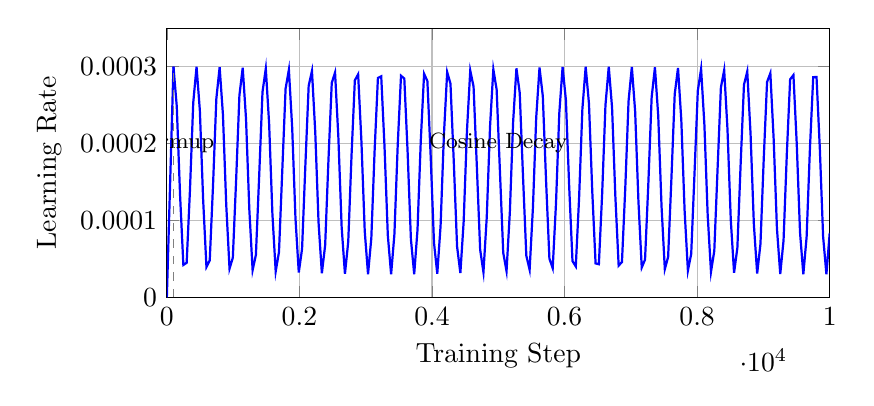
\begin{tikzpicture}
    \begin{axis}[
        width=10cm,
        height=5cm,
        xlabel={Training Step},
        ylabel={Learning Rate},
        xmin=0, xmax=10000,
        ymin=0, ymax=3.5e-4,
        grid=major,
        scaled y ticks=false,
        yticklabel style={
            /pgf/number format/fixed,
            /pgf/number format/precision=4
        },
    ]
        % Warmup phase
        \addplot[thick, blue, domain=0:100] {3e-4 * x / 100};

        % Cosine decay phase
        \addplot[thick, blue, domain=100:10000, samples=200]
            {3e-5 + (3e-4 - 3e-5) * (1 + cos(deg((x-100)/(10000-100) * 180))) / 2};

        % Annotations
        \node[font=\footnotesize] at (axis cs:50, 2e-4) {Warmup};
        \node[font=\footnotesize] at (axis cs:5000, 2e-4) {Cosine Decay};
        \draw[dashed, gray] (axis cs:100, 0) -- (axis cs:100, 3e-4);
    \end{axis}
\end{tikzpicture}
\caption{Learning rate schedule: linear warmup then cosine decay}
\label{fig:lr-schedule}
\end{figure}

\subsection{Implementation}

\begin{lstlisting}[style=python, caption={LR schedule from trainer.py}]
def get_lr(step: int, config: TrainConfig) -> float:
    """Cosine learning rate schedule with warmup."""
    # Warmup phase
    if step < config.warmup_steps:
        return config.learning_rate * (step / config.warmup_steps)

    # Cosine decay phase
    progress = (step - config.warmup_steps) / (
        config.max_steps - config.warmup_steps
    )
    min_lr = config.learning_rate * 0.1  # Decay to 10% of max

    return min_lr + (config.learning_rate - min_lr) * (
        1 + math.cos(math.pi * progress)
    ) / 2
\end{lstlisting}

\subsection{Why This Schedule?}

\begin{itemize}
    \item \textbf{Warmup}: Early training is unstable; small LR prevents divergence
    \item \textbf{High LR}: Enables fast learning in the middle
    \item \textbf{Decay}: Fine-grained optimization at the end
\end{itemize}

% -----------------------------------------------------------------------------
\section{The Complete Training Step}
% -----------------------------------------------------------------------------

Here's how all components come together:

\begin{lstlisting}[style=python, caption={Complete training step from trainer.py}]
def train(self) -> None:
    self.model.train()
    data_iter = iter(self.train_loader)

    for step in range(self.start_step, self.config.max_steps):
        # Update learning rate
        lr = get_lr(step, self.config)
        for param_group in self.optimizer.param_groups:
            param_group["lr"] = lr

        # Gradient accumulation loop
        self.optimizer.zero_grad()
        total_loss = 0.0

        for micro_step in range(self.config.gradient_accumulation_steps):
            batch = next(data_iter)
            batch = {k: v.to(self.device) for k, v in batch.items()}

            # Forward pass with mixed precision
            with autocast(enabled=self.mixed_precision):
                outputs = self.model(**batch)
                loss = outputs["loss"]
                loss = loss / self.config.gradient_accumulation_steps

            total_loss += loss.item()

            # Backward pass
            if self.scaler is not None:
                self.scaler.scale(loss).backward()
            else:
                loss.backward()

        # Gradient clipping and optimizer step
        if self.scaler is not None:
            self.scaler.unscale_(self.optimizer)

        grad_norm = torch.nn.utils.clip_grad_norm_(
            self.model.parameters(),
            self.config.grad_clip,
        )

        if self.scaler is not None:
            self.scaler.step(self.optimizer)
            self.scaler.update()
        else:
            self.optimizer.step()

        # Logging
        if step % self.config.log_interval == 0:
            self.log_metrics(step, total_loss, grad_norm, lr)
\end{lstlisting}

% -----------------------------------------------------------------------------
\section{Running Training}
% -----------------------------------------------------------------------------

\subsection{Using the CLI}

\begin{lstlisting}[style=shell]
# Train with default config
uv run trylm train

# Train with custom parameters
uv run trylm train \
    --config configs/tiny_stories.yaml \
    --batch-size 32 \
    --max-steps 5000 \
    --learning-rate 1e-4

# Resume from checkpoint
uv run trylm train --resume checkpoints/step_5000
\end{lstlisting}

\subsection{Expected Output}

\begin{lstlisting}[style=shell, numbers=none]
Training TryLM...
Device: cuda
Model parameters: 10,821,120

Step     0 | Loss: 10.234 | PPL: 27826 | LR: 0.00000 | Grad: 2.31
Step    10 | Loss:  9.456 | PPL: 12806 | LR: 0.00003 | Grad: 1.82
Step    20 | Loss:  8.123 | PPL:  3375 | LR: 0.00006 | Grad: 1.45
...
Step  1000 | Loss:  3.456 | PPL:    31 | LR: 0.00029 | Grad: 0.67
\end{lstlisting}

% -----------------------------------------------------------------------------
\section{Exercises}
% -----------------------------------------------------------------------------

\begin{exercise}
\textbf{Calculate Effective Batch Size}

With batch\_size=64, gradient\_accumulation\_steps=4, and 4 GPUs using data parallelism, what is the effective batch size?
\end{exercise}

\begin{exercise}
\textbf{Learning Rate Calculation}

For warmup\_steps=100, max\_steps=10000, and learning\_rate=3e-4:
\begin{enumerate}
    \item What is the LR at step 50?
    \item What is the LR at step 100?
    \item What is the LR at step 5000?
    \item What is the LR at step 9900?
\end{enumerate}
\end{exercise}

\begin{exercise}
\textbf{Gradient Clipping Experiment}

Train the same model with different grad\_clip values:
\begin{lstlisting}[style=shell, numbers=none]
uv run trylm train --max-steps 1000 --grad-clip 0.5
uv run trylm train --max-steps 1000 --grad-clip 1.0
uv run trylm train --max-steps 1000 --grad-clip 5.0
\end{lstlisting}

How does the training loss curve differ?
\end{exercise}

% -----------------------------------------------------------------------------
\section{Summary}
% -----------------------------------------------------------------------------

\begin{summary}
    \item The \textbf{training loop}: forward $\to$ backward $\to$ optimize $\to$ repeat
    \item \textbf{AdamW} with differential weight decay is standard for transformers
    \item \textbf{Gradient accumulation} enables larger effective batches than GPU memory allows
    \item \textbf{Mixed precision} (float16) speeds training and reduces memory
    \item \textbf{Gradient clipping} prevents exploding gradients
    \item \textbf{LR schedule}: warmup + cosine decay for stable, effective training
\end{summary}

Training is now running! In the next chapter, we'll learn how to monitor progress, save checkpoints, and ensure reproducibility.
